\documentclass[conference]{IEEEtran}
\IEEEoverridecommandlockouts

% preambulo:
\usepackage[utf8]{inputenc}
% caracteres utf8 (tildes, enie) sin tener que usar comandos


%% NO AGREGAR PAQUETES ANTES DE ESTO, ES IMPORTANTE QUE BABEL ESTE PRIMERO

%%%%%%%%%%%%%%%%%%%%%%%%%%%%%%%%%
%% PAQUETES EXTRA %%%%%%%%%%%%%%%
%%%%%%%%%%%%%%%%%%%%%%%%%%%%%%%%%

\usepackage{subfiles}

\usepackage{cite}
\usepackage{amsmath,amssymb,amsfonts}
\usepackage{algorithmic}
\usepackage{textcomp}
\usepackage{xcolor}

\usepackage{steinmetz} % comando \phase{}
\usepackage{units} % permite usar nicefrac
\usepackage{graphicx} % importar imagenes
\usepackage{float} % posicion H para floats
\usepackage[colorinlistoftodos]{todonotes}


\usepackage[a4paper, total={6in, 8in}]{geometry} 
% margenes correctos en subarchivos

\setlength{\parindent}{10pt}			%cuanta sangria al principio de un parrafo
\usepackage{indentfirst}				%pone sangria al primer parrafo de una seccion

\def\BibTeX{{\rm B\kern-.05em{\sc i\kern-.025em b}\kern-.08em
    T\kern-.1667em\lower.7ex\hbox{E}\kern-.125emX}}


%%%%%%%%%%%%%%%%%%%%%%%%%%%%%%%%%%%%%%%%%%%%%%%%%%%%%%%%%%%
%% NO AGREGAR PAQUETES DESPUES DE ESTO, ES IMPORTANTE QUE HYPERREF ESTE ULTIMO
\usepackage[hidelinks]{hyperref} % hipervinculos sin cajitas rojas

\usepackage[spanish, es-tabla, es-nodecimaldot]{babel} 
% texto automatico en espaniol
% "tabla" en vez de "cuadro"
% no reemplaza puntos decimales por comas

\usepackage{listings}
\usepackage{float}
\lstset{basicstyle=\small\ttfamily,columns=fullflexible}



\def\BibTeX{{\rm B\kern-.05em{\sc i\kern-.025em b}\kern-.08em
    T\kern-.1667em\lower.7ex\hbox{E}\kern-.125emX}}
\begin{document}

\title{Retoque fotográfico mediante reconstrucciones geométricas heurísticas}
\author{\IEEEauthorblockN{Ariel Nowik, Joaquin Mestanza, Rocio Parra, Martina Máspero, Marcelo Regueira}
\IEEEauthorblockA{22.05 - Análisis de Señales y Sistemas Digitales - Grupo 1} \\
\textit{ITBA: Instituto Tecnológico de Buenos Aires}\\
Ciudad de Buenos Aires, Argentina
}
\maketitle

\begin{abstract}
En este trabajo se estudiaron
 diversos métodos de retoque de imagenes para eliminar elementos no deseados presentes en diversas fuentes. Finalmente se procedió a realizar una implementación en función de las tecnicas analizadas seguida de un análisis de sus ventajas y desventajas.
\end{abstract}

\section{Introducción}
Las imágenes son utilizadas diariamente para transmitir distintos tipos de información, desde un anuncio hasta una fotografía, o incluso en un instructivo para el armado de un objeto desmontable. Nos permiten en estos casos interpretar más fácilmente la información que el emisor nos quiere transmitir, que si lo hiciera sólo a través de texto.\par
En algunos casos la imagen en cuestión puede estar comprimida, contener ruido, o poseer otra característica que implique una calidad más deficiente. En consecuencia, no cumpliría en forma óptima con el objetivo de transmitir la información original. De entre todos los tipos, la característica que se tratará será la presencia de un objeto no deseado en la imagen, y su eliminación.\par
Se puede pensar en una imagen que representa un espacio determinado, conteniendo diferentes objetos (como un escritorio con útiles). 
\begin{figure}[!ht]
\begin{centering}
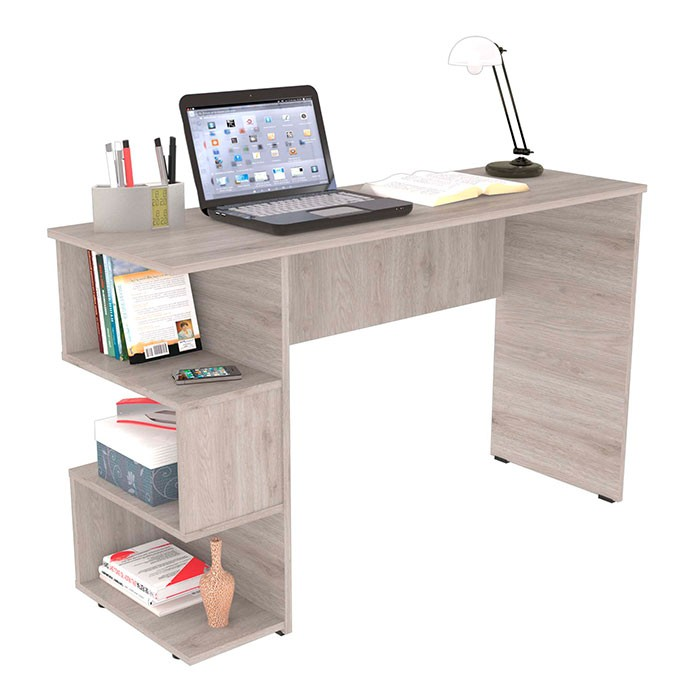
\includegraphics[scale=0.2]{ImagenesAux/desktop.jpg}
\par\end{centering}
\caption{Escritorio genérico}
\end{figure}
Naturalmente no es posible ``adivinar'' lo que se encuentra por detrás de ellos (que en principio podría ser parte del escritorio), ya que requiere información adicional (como por ejemplo, el escritorio sin los útiles), la cual en principio no es accesible. Por lo tanto la idea es, de algún modo estimar la zona de la imagen que contiene el objeto no deseado utilizando el resto de la misma. En lo que sigue de este trabajo describiremos con mayor detalle diversos métodos para llevar a cabo este proceso.
%asimilar la zona de la imagen a reemplazar con el resto de la misma.% 

\section{Alternativas exploradas}

\subsection{Exemplar-based image inpainting}


\begin{thebibliography}{00}
\bibitem{b1} A. Criminisi, P. Perez, and K. Toyama, “Region filling and object
removal by exemplar-based image inpainting,” IEEE T. Image Process.,
vol. 13, no. 9, pp. 1200–1212, Sep. 2004.

\bibitem{b2} Pierre Buyssens, Maxime Daisy, David Tschumperlé, Olivier Lézoray. Exemplar-based Inpainting:
Technical Review and new Heuristics for better Geometric Reconstructions. IEEE Transactions on
Image Processing, Institute of Electrical and Electronics Engineers, 2015, 24 (6), pp.1809 - 1824.
ff10.1109/TIP.2015.2411437ff. ffhal-01147620f
\end{thebibliography}
\end{document}
